\documentclass[11pt,a4paper]{article}

\usepackage[utf8]{inputenc}
\usepackage[T1]{fontenc}
\usepackage{amsmath,amssymb}
\usepackage{graphicx}
\usepackage{booktabs}
\usepackage{tabularx}
\usepackage{array}
\usepackage{changepage}
\usepackage{hyperref}
\usepackage{cleveref}
\usepackage[numbers,sort&compress]{natbib}

% Centered, text-wrapping tabularx column, used to keep wide comparison
% tables exactly \textwidth-aligned instead of overflowing the margin.
\newcolumntype{Y}{>{\centering\arraybackslash}X}

\title{State-of-the-art and Critical Analysis of Quantum-Inspired\\
Evolutionary Algorithms for Multi-Objective Optimization:\\
Taxonomy, Features, and Limitations}
\author{TODO: author list}
\date{\today}

\begin{document}

\maketitle

\begin{abstract}
% TODO: write abstract once Sections 3-6 have stable content.
\end{abstract}

\section{Introduction}
\label{sec:introduction}

% TODO: motivation for surveying quantum-inspired evolutionary algorithms
% (QIEA) applied to multi-objective optimization (MOO).

\subsection{Scope and Inclusion Criteria}
\label{sec:introduction:scope}
% TODO: define the literature search scope and inclusion/exclusion
% criteria for the survey (databases searched, date range, keywords).

\subsection{Contributions}
\label{sec:introduction:contributions}
% TODO: list this survey's contributions (taxonomy, feature comparison,
% critical analysis, case study).

\subsection{Paper Organization}
\label{sec:introduction:organization}
% TODO: one paragraph outlining Sections~\ref{sec:background}-\ref{sec:conclusion}.

\section{Background}
\label{sec:background}

\subsection{Quantum Computing Concepts for QIEA}
\label{sec:background:quantum}

Quantum-inspired evolutionary algorithms borrow their representation and
update rules from the mathematics of a single qubit, without requiring
quantum hardware to run. A qubit's state is a normalized superposition of
the two classical basis states,
\begin{equation}
  \label{eq:qubit}
  \lvert\psi\rangle = \alpha\lvert 0\rangle + \beta\lvert 1\rangle,
  \qquad \lvert\alpha\rvert^2 + \lvert\beta\rvert^2 = 1,
\end{equation}
where $\lvert\alpha\rvert^2$ and $\lvert\beta\rvert^2$ are interpreted as
the probability of the qubit collapsing to $0$ or $1$ upon observation.
\citet{han2002qea} introduced the \emph{Q-bit chromosome}: an individual
is encoded not as a fixed binary string but as a string of such
probability-amplitude pairs $(\alpha_i,\beta_i)$, one per bit position.
Observing (measuring) a Q-bit chromosome collapses it into an ordinary
binary solution that can be evaluated by the problem's fitness function,
while the amplitudes themselves are what the algorithm evolves --
maintaining, in effect, a probabilistic superposition over the whole
population's search history rather than a single discrete solution.

The corresponding variation operator is the \emph{Q-gate}, a rotation
applied to each Q-bit's amplitude pair,
\begin{equation}
  \label{eq:qgate}
  \begin{pmatrix}\alpha_i'\\ \beta_i'\end{pmatrix}
  =
  \begin{pmatrix}\cos\theta_i & -\sin\theta_i\\ \sin\theta_i & \cos\theta_i\end{pmatrix}
  \begin{pmatrix}\alpha_i\\ \beta_i\end{pmatrix},
\end{equation}
where the rotation angle $\theta_i$ and its sign are looked up from a
predetermined table that compares the current bit's observed value and
fitness contribution against the best solution found so far, nudging the
amplitude pair toward whichever basis state that comparison favors. This
rotation-gate mechanism is what most surveyed QIEA methods share
regardless of application domain~\citep{vivek2025fss}, and it is the
representation/operator combination
Section~\ref{sec:taxonomy:representation} and
Section~\ref{sec:taxonomy:operator} use as the taxonomy's reference
point; variants that replace or augment it with interference- or
entanglement-inspired operators are discussed there rather than here.

\subsection{Multi-Objective Optimization Fundamentals}
\label{sec:background:moo}

A multi-objective optimization problem (MOP) seeks to simultaneously
optimize $m \geq 2$ objective functions
$f_1(x), \dots, f_m(x)$ over a decision space $x \in \Omega$. Because the
objectives typically conflict, there is generally no single $x$ that
minimizes (or maximizes) all of them at once; instead, a solution
$x_1$ is said to \emph{Pareto-dominate} $x_2$ if $x_1$ is at least as
good as $x_2$ on every objective and strictly better on at least one. A
solution is \emph{Pareto-optimal} if no other feasible solution
dominates it, and the image of the set of all Pareto-optimal solutions
in objective space is the \emph{Pareto front}. Rather than a single best
answer, a multi-objective evolutionary algorithm (MOEA) therefore aims to
return a population that approximates this front as closely and as
evenly as possible~\citep{emmerich2018tutorial}.

Comparing how well two algorithms' output populations approximate the
true (or best-known) Pareto front requires quality indicators that
capture both convergence and diversity, since neither alone is
sufficient: a tightly clustered set of points on the front converges well
but covers it poorly, while a widely spread set may cover a region no
solution actually dominates. The indicators used throughout this
survey are:
\begin{itemize}
  \item \textbf{Hypervolume (HV)}: the volume of objective space
    dominated by a solution set relative to a fixed reference point --
    the only indicator that is strictly monotonic with Pareto dominance
    on its own, and the basis of hypervolume-driven selection in
    SMS-EMOA~\citep{beume2007smsemoa}. Its value is sensitive to the
    reference point and normalization used, a methodological detail
    Section~\ref{sec:case-study:hypervolume} returns to.
  \item \textbf{Inverted Generational Distance (IGD)}: the average
    distance from each point on a reference (true or best-known) Pareto
    front to its nearest neighbor in the algorithm's output set,
    rewarding both convergence and coverage but requiring that reference
    front to be known or well-approximated -- a requirement this
    survey's own case study (Section~\ref{sec:case-study}) does not
    meet for any of its benchmark circuit families, so IGD does not
    itself recur there.
  \item \textbf{Spread and spacing}: measures of how evenly solutions are
    distributed along the approximated front, independent of how close
    that front is to the true optimum. Spread recurs in the case study
    (Section~\ref{sec:case-study:algorithms}); spacing does not.
\end{itemize}
See \citet{emmerich2018tutorial} and \citet{hanne2025review} for a fuller
treatment of these fundamentals and their formal definitions.

\subsection{Classical MOEAs}
\label{sec:background:moea}

The Pareto-dominance-based family of MOEAs -- the family every QIEA-MOO
method surveyed here either builds on or is benchmarked against -- traces
back to \citet{schaffer1985vega}'s Vector Evaluated Genetic Algorithm
(VEGA), which optimized each objective in a separate sub-population and
suffered from poor diversity as a result. Successive algorithms
addressed this diversity problem in turn: \citet{fonseca1993moga}'s MOGA
introduced Pareto-rank-based fitness with fitness sharing;
\citet{horn1994npga}'s NPGA added dominance-based tournament selection
with niching; \citet{zitzler1999spea}'s SPEA introduced an external
archive of non-dominated solutions and strength-based fitness;
\citet{knowles2000paes}'s PAES took a different design point entirely,
a $(1+1)$ evolution strategy with no population or crossover, using an
adaptive grid archive for diversity; and
\citet{corne2000pesa,corne2001pesa2}'s PESA and PESA-II introduced a
hyper-grid (``hyperbox'') archive with selection performed at the
hyperbox level. This lineage matters for QIEA-MOO specifically because
several surveyed methods graft a Q-bit/Q-gate representation onto one of
these selection mechanisms rather than inventing a new one --
understanding the mechanism being reused is a precondition for the
taxonomy's hybridization axis (Section~\ref{sec:taxonomy:hybridization}).

Five classical MOEAs recur most often as the baselines QIEA-MOO methods
are compared against in the surveyed literature, and this survey adopts
the same five as its background reference set:
\begin{itemize}
  \item \textbf{NSGA-II}~\citep{deb2002nsga2}: fast non-dominated
    sorting (ranking the population into successive Pareto fronts) combined
    with crowding-distance-based diversity preservation within each
    front; the most widely used MOEA baseline, and the one this survey's
    own case-study pipeline builds on (Section~\ref{sec:case-study}).
  \item \textbf{NSGA-III}~\citep{debjain2014nsga3}: replaces
    crowding distance with reference-point-based niching, extending
    NSGA-II's non-dominated-sorting framework to many-objective problems
    ($m \gg 3$) where crowding distance alone provides insufficient
    selection pressure.
  \item \textbf{SPEA2}~\citep{zitzler2001spea2}: refines SPEA with a
    finer-grained strength-based fitness assignment, a $k$-th-nearest-
    neighbor density estimator, and a fixed-size external archive.
  \item \textbf{MOEA/D}~\citep{zhangli2007moead}: decomposes the
    multi-objective problem into a set of scalar subproblems via weight
    vectors, solving them cooperatively using neighborhood information --
    a fundamentally different, decomposition-based design point from the
    three Pareto-dominance-based algorithms above.
  \item \textbf{SMS-EMOA}~\citep{beume2007smsemoa}: an indicator-based
    method whose environmental selection removes whichever individual
    contributes least to the population's dominated hypervolume, directly
    optimizing for the HV indicator described in
    Section~\ref{sec:background:moo} rather than a proxy for it.
\end{itemize}
Together these five span the main selection paradigms QIEA-MOO methods
adopt or compare against: crowding-distance-based, reference-point-based,
strength/density-based, decomposition-based, and hypervolume-driven.
Section~\ref{sec:taxonomy:selection} uses this same set of paradigms as
one of the taxonomy's classification axes.

\section{Taxonomy}
\label{sec:taxonomy}

% TODO: introduce the classification axes below and how they were derived
% from the surveyed literature (first draft, not yet validated against a
% systematic literature pass -- see journal.txt).

\subsection{Representation Scheme}
\label{sec:taxonomy:representation}

\subsection{Quantum-Inspired Operator Type}
\label{sec:taxonomy:operator}
% TODO: rotation gate vs. interference vs. entanglement-inspired operators.

\subsection{Selection and Diversity Mechanism}
\label{sec:taxonomy:selection}

\subsection{Hybridization with Classical MOEAs}
\label{sec:taxonomy:hybridization}

\subsection{Application Domain}
\label{sec:taxonomy:application}

\section{Feature Comparison}
\label{sec:feature-comparison}

Section~\ref{sec:taxonomy} introduced five classification axes and
applied them narratively to the QIEA-for-MOO methods identified so far.
This section applies the same axes systematically, one row per method,
across two tables: Table~\ref{tab:feature-comparison-taxonomy} recaps
representation, operator type, selection mechanism, and application
domain (the four axes for which the notes gathered while building
Section~\ref{sec:background}'s and Section~\ref{sec:taxonomy}'s
citations already give a confident answer), and
Table~\ref{tab:feature-comparison-performance} turns to complexity,
scalability, convergence behavior, benchmarks, and reported performance
-- the dimensions this survey's contributions
(Section~\ref{sec:introduction:contributions}) also promise to cover.

A methodological caveat applies to Table~\ref{tab:feature-comparison-performance}
specifically, and is itself a preview of
Section~\ref{sec:critical-analysis}'s reproducibility discussion: at
this drafting stage, several of its cells reflect only what each
method's title, abstract, and this survey's own literature-gathering
notes state, not an independent re-derivation or reproduction of the
original results. Cells that would require reading the full paper to
state with confidence are marked accordingly rather than filled with an
unverified number, following the same verify-before-citing discipline
already applied to every entry in this survey's bibliography. That so
many cells resist confident filling from title/abstract alone, for a
comparison table that is supposed to be the survey's most concrete
deliverable, is itself early evidence for a pattern
Section~\ref{sec:critical-analysis} treats as a cross-cutting limitation:
QIEA-MOO papers routinely under-report the complexity, scale, and
statistical rigor of their own evaluations relative to what a reader
would need to compare them fairly against one another.

\begin{table}[htbp]
  \centering
  \small
  \caption{Representation, operator, selection, and domain summary of
    the surveyed QIEA-MOO methods (recap of the taxonomy axes,
    Section~\ref{sec:taxonomy}).}
  \label{tab:feature-comparison-taxonomy}
  \begin{adjustwidth}{-2cm}{-2cm}
  \centering
  \begin{tabularx}{\linewidth}{@{}p{2.1cm}XXXX@{}}
    \toprule
    Method & Representation & Quantum-Inspired Operator(s) & Selection /
    Diversity & Application Domain \\
    \midrule
    QMEA~\citep{kim2006qmea} &
      Q-bit chromosome, observed to a binary decision vector &
      Rotation-gate update only &
      Direct Pareto-dominance ranking (no crowding distance) &
      Multi-objective 0/1 knapsack (combinatorial) \\
    QNSGA-II~\citep{guzel2022qnsga2} &
      Q-bit chromosome layered onto an NSGA-II individual &
      Rotation gate + superposition-based sampling &
      NSGA-II crowding distance, unmodified &
      General-purpose multi-objective benchmarks (not itemized in
      abstract-level notes) \\
    Continuous QIEA-MOO~\citep{olvera2023continuous} &
      Q-bit angle decoded to a real-valued decision variable &
      Rotation gate &
      Compared directly against NSGA-II as an external baseline &
      Continuous-space multi-objective benchmark problems \\
    EAH-QNSGA-II~\citep{kumar2026eahqnsga2} &
      Q-bit chromosome layered onto an NSGA-II individual &
      Adaptive rotation gate + entanglement-driven crossover +
      post-hoc local search &
      NSGA-II crowding distance, unmodified &
      Electric-vehicle charging-station siting (real-world
      infrastructure) \\
    QIEA-MOO for waste collection~\citep{gilea2026waste} &
      Not yet confirmed against full text (self-citation; venue/DOI
      itself unconfirmed, see the bibliography note) &
      Not yet confirmed against full text &
      Not yet confirmed against full text &
      Waste-collection vehicle routing (real-world logistics) \\
    \bottomrule
  \end{tabularx}
  \end{adjustwidth}
\end{table}

\begin{table}[htbp]
  \centering
  \small
  \caption{Complexity, scalability, convergence, and reported
    performance of the surveyed QIEA-MOO methods. Cells marked
    ``not confirmed'' require reading the full paper, not just its
    abstract, before any specific claim is cited (see the methodological
    caveat above).}
  \label{tab:feature-comparison-performance}
  \begin{adjustwidth}{-2cm}{-2cm}
  \centering
  \begin{tabularx}{\linewidth}{@{}p{2.1cm}XXXX@{}}
    \toprule
    Method & Complexity & Scalability & Convergence & Reported
    Performance \\
    \midrule
    QMEA~\citep{kim2006qmea} &
      Not confirmed; direct Pareto ranking without NSGA-II's fast
      non-dominated sort suggests a per-generation cost at or above
      NSGA-II's, not below it &
      Evaluated only on the knapsack instance sizes used in the
      original paper; not confirmed &
      Not confirmed &
      Not confirmed beyond the paper's own framing as an early
      QIEA-MOO proof of concept \\
    QNSGA-II~\citep{guzel2022qnsga2} &
      Inherits NSGA-II's per-generation non-dominated-sorting cost,
      since selection is left unmodified (Section~\ref{sec:taxonomy:selection});
      the superposition-sampling step adds low-order per-Q-bit overhead &
      Not confirmed &
      Reported to converge faster than a plain NSGA-II baseline; the
      magnitude and statistical significance of that claim are not
      independently confirmed here &
      Improved convergence speed relative to NSGA-II (self-reported) \\
    Continuous QIEA-MOO~\citep{olvera2023continuous} &
      Not confirmed &
      Not confirmed &
      Directly compared against NSGA-II on shared continuous benchmark
      problems, per the paper's own framing, but the direction and size
      of any advantage are not confirmed here &
      Not confirmed beyond the paper's framing as a head-to-head
      comparison against NSGA-II \\
    EAH-QNSGA-II~\citep{kumar2026eahqnsga2} &
      Inherits NSGA-II's per-generation cost plus entanglement-crossover
      and local-search overhead; the local-search pass is structurally
      analogous to the hybrid-LAS refinement in this survey's own case
      study (Section~\ref{sec:case-study:mutation}), applied after the
      main GA loop rather than during it &
      Evaluated on a single real-world EV-charging-siting case study;
      scaling behavior beyond that instance not confirmed &
      Not confirmed &
      Reports improved siting trade-offs on its case study relative to
      baseline planning approaches; specific metrics not confirmed here \\
    QIEA-MOO for waste collection~\citep{gilea2026waste} &
      Not confirmed &
      Not confirmed &
      Not confirmed &
      Not confirmed \\
    \bottomrule
  \end{tabularx}
  \end{adjustwidth}
\end{table}

Read across both tables, two patterns stand out even before the
critical analysis proper (Section~\ref{sec:critical-analysis}). First,
every method with a confirmed selection mechanism reuses NSGA-II's
crowding distance unmodified (Table~\ref{tab:feature-comparison-taxonomy}),
so any complexity or scalability claim that does exist is really a
claim about NSGA-II's own well-studied $O(MN^2)$ non-dominated-sorting
cost~\citep{deb2002nsga2} plus a low-order quantum-operator overhead --
none of the surveyed methods has been evaluated against a
selection mechanism whose asymptotic behavior differs enough from
NSGA-II's to matter at scale. Second, reported performance in this
literature is consistently self-comparative (a proposed method against
a classical NSGA-II baseline, run once per paper) rather than
cross-compared against the other QIEA-MOO methods in the same table --
no two of the four confirmed methods above are benchmarked against each
other anywhere in the sources gathered for this survey. Both
observations recur as cross-cutting limitations in
Section~\ref{sec:critical-analysis:cross-cutting}.

\section{Critical Analysis and Limitations}
\label{sec:critical-analysis}

\subsection{Per-Category Weaknesses}
\label{sec:critical-analysis:per-category}

This subsection revisits each of the five taxonomy axes from
Section~\ref{sec:taxonomy} in turn, this time asking not how the
surveyed methods differ along that axis but what limitation the axis
itself exposes once the methods are compared against each other.

\textbf{Representation.} The Q-bit chromosome transfers cleanly to
combinatorial 0/1 problems~\citep{kim2006qmea} but has no single
standard decoding convention for continuous decision spaces: where a
binary problem simply observes each Q-bit, \citet{olvera2023continuous}
must instead choose a specific interval mapping from rotation angle to
real value, a design decision with no equivalent in the original
formalism~\citep{han2002qea} to constrain it. Two papers that both
describe themselves as using ``the Q-bit representation'' may therefore
be doing meaningfully different things once a continuous problem is
involved, which weakens how much a shared representation label actually
tells a reader trying to compare methods across domains. Compounding
this, \citet{vivek2025fss}'s own survey of QIEA operators finds the
representation used almost exclusively on combinatorial or binary
problems (feature subset selection foremost among them); the continuous
adaptation remains comparatively rare and non-standardized, which limits
how confidently ``the Q-bit representation'' can be described as a
general-purpose MOO representation rather than one best suited to
combinatorial problems specifically.

\textbf{Quantum-inspired operator type.} Section~\ref{sec:taxonomy:operator}
already noted that interference, named alongside superposition and
entanglement as a general source of QIEA design inspiration
(Section~\ref{sec:introduction}), has no dedicated implementation in the
methods surveyed here. Taken together with how much of each surveyed
method's actual variation step reduces to the single rotation-gate
update rule from \citet{han2002qea} -- superposition-based sampling in
\citet{guzel2022qnsga2} and entanglement-driven crossover in
\citet{kumar2026eahqnsga2} are each one additional operator layered on
top of, not a replacement for, that same rotation gate -- this raises a
concrete risk for the field: that ``quantum-inspired'' is doing more
rhetorical work in motivating a paper's framing than algorithmic work in
its actual contribution, since the operator-type axis in practice offers
much less diversity than the three-phenomenon (superposition,
interference, entanglement) framing common in this literature's
introductions would suggest.

\textbf{Selection and diversity mechanism.} Every method in the
surveyed set with a confirmed selection mechanism inherits NSGA-II's
crowding distance unmodified
(Section~\ref{sec:taxonomy:selection}), and none pairs the Q-bit
representation with NSGA-III's reference-point niching, SPEA2's
density estimator, MOEA/D's decomposition, or SMS-EMOA's
hypervolume-driven selection. This concentration is worth weighing
against results that postdate most of the surveyed
QIEA-MOO papers: \citet{deng2025nsga3guarantees} give NSGA-III the first
proven approximation guarantees of its lineage, and
\citet{alghouass2025spea2beatsnsga2} prove SPEA2 achieves a
polynomial-time-optimal approximation of the Pareto front on a
benchmark problem where NSGA-II's best proven guarantee is only
roughly a factor of two. Neither result implies NSGA-II's
crowding-distance selection is a poor empirical choice in general, and
neither has been evaluated in combination with a Q-bit representation
specifically -- but they do mean the QIEA-MOO literature surveyed here
settled early and almost uniformly on one selection paradigm without the
benefit of the theoretical grounding that later became available for
comparing it against its main alternatives.

\textbf{Hybridization with classical MOEAs.} Hybridization in the
surveyed literature is uniformly shallow in the same direction: a Q-bit
representation and one or two quantum-inspired operators are grafted
onto an otherwise unmodified classical MOEA loop
(Section~\ref{sec:taxonomy:hybridization}), rather than the classical
algorithm's selection or archiving logic itself being redesigned around
what a quantum-inspired representation makes available (for instance,
using the amplitude pair's own uncertainty as a diversity signal, rather
than only its observed bit value). A second, related weakness is
evaluative rather than architectural: as already noted from
Table~\ref{tab:feature-comparison-performance}
(Section~\ref{sec:feature-comparison}), every reported performance claim
in the surveyed set compares the proposed method against a classical
NSGA-II baseline, and no two of the surveyed QIEA-MOO methods are
benchmarked against each other anywhere in the sources gathered for this
survey. A field in which every new method is shown to beat the same
baseline, but never compared against its own siblings, cannot yet
support a claim about which hybridization choice is preferable within
the QIEA-MOO cluster itself.

\textbf{Application domain.} The application domains covered split into
two disjoint clusters with no overlap
(Section~\ref{sec:taxonomy:application}): quantum-inspired algorithms
applied to classical combinatorial or engineering
problems~\citep{kim2006qmea,kumar2026eahqnsga2,gilea2026waste}, and
classical (non-quantum-inspired) algorithms applied to a genuinely
quantum problem domain, as in this survey's own case study
(Section~\ref{sec:case-study}) and its foundational
reference~\citep{ghlib2026scalable}. Within the first cluster, each
paper additionally validates on a single problem or a single real-world
instance -- one knapsack benchmark, one EV-charging-siting case study,
one waste-collection routing scenario -- rather than a shared benchmark
suite spanning multiple problem sizes or domains, so claims of general
applicability rest on a narrower evidentiary base than the breadth of
domains represented across the cluster as a whole might suggest.

\subsection{Cross-Cutting Open Problems}
\label{sec:critical-analysis:cross-cutting}

Three problems recur across every taxonomy category above rather than
being specific to one of them.

\textbf{Reproducibility gaps.} Building
Table~\ref{tab:feature-comparison-performance}
(Section~\ref{sec:feature-comparison}) directly surfaced this problem:
several of its complexity, scalability, and convergence cells could not
be filled with confidence from each paper's title and abstract alone,
and were marked accordingly rather than guessed at. This is not merely
a limitation of how this survey gathered its literature -- it reflects
that the information needed to independently reproduce or even
carefully re-derive a QIEA-MOO paper's headline result is often not
recoverable without the full paper and, in many cases, code or data
that may never have been released. This survey's own case study offers
a cautionary illustration of how easily such gaps can hide even inside
a codebase under active, careful maintenance: two real bugs in its
inter-block gate injection stage silently distorted every quantitative
fidelity result reported over several weeks of work, and were only
caught and fixed once the pipeline's output was checked against a
specific, otherwise-unremarkable circuit family
(Section~\ref{sec:case-study:pipeline}). If a reproducibility gap of
that kind can persist for weeks inside one actively-maintained pipeline
with its own test suite, the equivalent risk across independently
authored papers with no shared code and no obligation to re-verify a
predecessor's numbers before building on them is considerably harder to
rule out, not easier.

\textbf{Weak benchmarking practices.} The self-comparative-only pattern
already noted under hybridization above -- every method benchmarked
against NSGA-II, never against a sibling QIEA-MOO method -- is itself an
instance of a broader benchmarking weakness: comparisons in this
literature are run once, against one baseline, on one problem or
instance, without the kind of multi-seed statistical treatment that
would distinguish a genuine improvement from run-to-run variance. This
survey's own case study underscores why that treatment matters: an
early quantitative finding in the project's own results, later
retracted, turned out to be a measurement artifact rather than a real
algorithmic effect once re-measured carefully
(Section~\ref{sec:case-study:algorithms}) -- exactly the kind of error a
single-run, single-baseline comparison is poorly positioned to catch.
Compounding this, the classical baselines this literature compares
against have themselves only recently acquired the kind of formal
scrutiny that would let such comparisons be interpreted rigorously:
\citet{opris2024nsga3runtime} and \citet{deng2025nsga3guarantees}'s
runtime and approximation-guarantee analyses of NSGA-III, and
\citet{alghouass2025spea2beatsnsga2}'s analogous result for SPEA2, all
postdate nearly every QIEA-MOO paper surveyed here, so those papers'
original empirical comparisons against NSGA-II could not have accounted
for guarantees that did not yet exist.

\textbf{Scalability claims rarely stress-tested.} Every application
example in Section~\ref{sec:critical-analysis:per-category}'s
application-domain discussion is evaluated at a single scale rather than
across a size sweep, so a method's reported performance says little
about how it would behave on a substantially larger instance of the same
problem. This survey's own case study again illustrates the point
concretely, on the quantum-circuit-optimization side rather than the
QIEA-MOO side: its own fidelity-estimation subsystem required distinct,
per-circuit-family scaling fixes and qubit-count ceilings before it
could be trusted at all beyond small instances
(Section~\ref{sec:case-study:pipeline}), a cost that a single-scale
evaluation would never have surfaced. Sweeping across scale within the
case study's own 225-run core baseline (Section~\ref{sec:case-study:algorithms})
surfaces a second, sharper instance of the same point: mean
\texttt{fidelity\_final} \emph{declines} with qubit count for four of
the five circuit families tested (e.g.\ \texttt{qft}: 0.070 at $n{=}8$,
0.015 at $n{=}12$, 0.0005 at $n{=}20$; \texttt{hw\_efficient\_ansatz}:
0.098, 0.020, 0.0004 over the same sizes), while the fifth,
\texttt{weak\_random}, instead \emph{improves} with qubit count (0.225,
0.363, 0.375), as Figure~\ref{fig:scaling-fidelity} shows directly. A
single-scale evaluation of any one of these families
-- exactly the evaluative pattern this subsection has already flagged
as the norm in the QIEA-MOO literature surveyed above -- would report
only one point on what is evidently not even a consistent trend across
problem instances, let alone across algorithms. We do not attempt to
adjudicate here whether the declining trend reflects a genuine scaling
limitation of the pipeline or simply the exact fidelity metric's own
well-known exponential contraction toward zero for two generically
different unitaries as $n$ grows
(Section~\ref{sec:background:quantum}) -- distinguishing the two is
exactly the kind of question the separate, forthcoming empirical
results paper is responsible for answering, not this survey.

\begin{figure}[htbp]
  \centering
  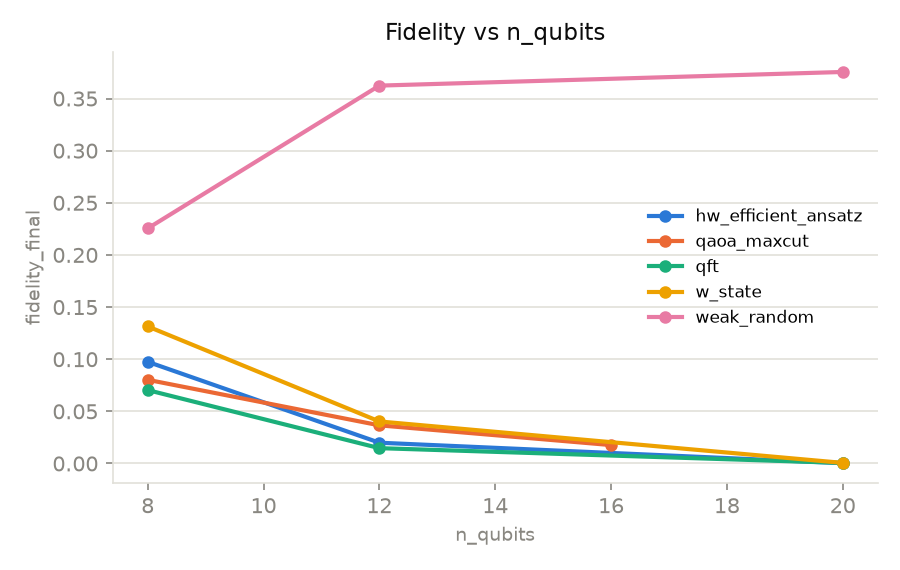
\includegraphics[width=0.75\linewidth]{figures/scaling_fidelity.png}
  \caption{Mean \texttt{fidelity\_final} vs.\ qubit count, per circuit
    family, pooled across the three per-block optimizers of the
    225-run core baseline (Section~\ref{sec:case-study:algorithms}).
    Four of five families decline toward the metric's near-zero floor
    as $n$ grows; \texttt{weak\_random} is the exception. A single-scale
    evaluation of any one family in isolation -- the norm in the
    QIEA-MOO literature surveyed above -- would surface only one point
    on this plot.}
  \label{fig:scaling-fidelity}
\end{figure}

More fundamentally, the
Pareto-dominance relation every classical MOEA baseline in
Section~\ref{sec:background:moea} and every NSGA-II-hybridized QIEA-MOO
method in Section~\ref{sec:taxonomy:hybridization} relies on has itself
only recently been shown to have a structural weakness --
\citet{zheng2025weakparetoboundary}'s ``weak Pareto boundary'' result --
that predates none of the surveyed QIEA-MOO literature's own
publication dates and so could not have been accounted for by any of
it. Scalability claims in this field, in short, rest on baselines and
dominance relations whose own limits are still being discovered, on top
of application-side evaluations that rarely test more than one problem
scale to begin with.

\section{Case Study: Block-Partitioned Quantum Circuit Optimization}
\label{sec:case-study}

% TODO: illustrative use of the project's own pipeline (partition ->
% per-block MOO -> inter-block injection -> compression, see
% M1\_finale/final\_m1\_script.py) to ground abstract taxonomy claims in a
% concrete worked example. Framed explicitly as illustrative, not as this
% paper's primary evidence -- full empirical validation is deferred to the
% planned separate empirical results paper.
%
% IMPORTANT: any number cited here must be re-verified on the
% post-2026-09-04 injection-stage-bug-fix codebase before being written
% down -- see logs.txt's "CURRENT STATUS OF RESULTS" section. Do not copy
% pre-fix figures into this section.

\subsection{Pipeline Overview}
\label{sec:case-study:pipeline}
% TODO: brief description of the partition/optimize/inject/compress
% pipeline for readers of the survey (not a full method section -- that
% belongs to the separate empirical paper).

\subsection{NSGA-II vs.\ SMS-EMOA vs.\ NSGA-III as a Worked Example}
\label{sec:case-study:algorithms}
% TODO: use the three interchangeable per-block optimizers as a concrete
% illustration of crowding-distance vs.\ hypervolume-driven vs.\
% reference-point selection trade-offs (Section~\ref{sec:taxonomy:selection}).

\subsection{No Universally-Best Mutation Operator}
\label{sec:case-study:mutation}
% TODO: the project's mutation-scheme ablation (point / swap\_add /
% swap\_add\_delete) as a concrete instance of a taxonomy/limitations
% claim. Pending re-run on the fixed injection-stage code.

\subsection{Hypervolume Comparability Across Algorithms}
\label{sec:case-study:hypervolume}
% TODO: adaptive vs.\ fair/shared-reference hypervolume as an illustration
% of the benchmarking-practice limitations raised in
% Section~\ref{sec:critical-analysis:cross-cutting}. This finding is
% structural (about how HV is computed), not tied to the injection-stage
% bug fix, so it can be cited as-is -- see logs.txt's "HYPERVOLUME
% COMPARABILITY ACROSS ALGORITHMS" section.

\section{Open Challenges and Future Directions}
\label{sec:open-challenges}

Section~\ref{sec:critical-analysis} looked backward: what the surveyed
QIEA-for-MOO literature and this survey's own case study already show
to be weak or under-tested. This section looks forward, organized into
four groups -- the two open questions this survey's own analysis raised
without answering, methodological directions for QIEA-MOO as a field,
technical extensions specific to the case-study pipeline, and the
broader trajectory the field appears to be moving toward.

\subsection{Open Questions Raised by This Survey}
\label{sec:open-challenges:raised}

Two specific questions surfaced earlier in this survey without being
resolved, and we restate them here as concrete starting points rather
than let them dissolve into the more general directions below.

First, Section~\ref{sec:taxonomy:application} found the application
domains covered by the surveyed literature split into two disjoint
clusters -- quantum-inspired algorithms applied to classical
combinatorial or engineering problems, and classical (non-quantum-
inspired) algorithms applied to a genuinely quantum problem domain, as
in this survey's own case study -- with no method in the literature
gathered so far combining both: a Q-bit-represented, quantum-inspired
MOEA applied directly to a quantum-computing problem domain such as
circuit optimization or compilation. Concretely, this would mean
encoding a gate sequence itself as a string of Q-bit amplitude pairs,
with rotation-gate (and perhaps entanglement- or interference-inspired)
operators evolving that encoding directly, rather than -- as this
survey's own case study does -- using an ordinary classical chromosome
of gate tuples inside a classical MOEA. Whether such a representation
would offer any advantage over either cluster alone (e.g.\ a more
natural search-space geometry for gate sequences, given that both
objects are already expressed in the language of qubits and rotations)
is, to our knowledge, untested anywhere in the current literature.

Second, Section~\ref{sec:case-study:hypervolume} found that NSGA-III's
Pareto front is not only smaller than NSGA-II's or SMS-EMOA's under a
shared-reference (fair) hypervolume comparison in this project's own
pipeline, but increasingly so as problem size grows. We could state
\emph{that} finding with confidence; we could not state \emph{why}
without further investigation reaching beyond survey scope --
specifically, whether it traces to Deb and Jain's reference-point
niching providing systematically less selection pressure toward a
front's extremes than crowding distance or hypervolume-driven
environmental selection do, as this pipeline's block sizes grow, or to
some interaction specific to this pipeline's block-partitioned setting
that would not generalize to non-partitioned NSGA-III use. Distinguishing
these is exactly the kind of question the separate, forthcoming
empirical results paper is positioned to pursue, since it requires
running controlled ablations this survey does not.

\subsection{Methodological Directions for QIEA-MOO}
\label{sec:open-challenges:methodological}

Several of Section~\ref{sec:critical-analysis:per-category}'s
per-category weaknesses point directly at concrete methodological gaps
rather than only diagnosing a problem. The selection-mechanism
concentration on NSGA-II's crowding distance
(Section~\ref{sec:taxonomy:selection}) is the clearest: no surveyed
method has paired the Q-bit representation with NSGA-III's
reference-point niching, SPEA2's density estimator, MOEA/D's
decomposition, or SMS-EMOA's hypervolume-driven selection, so which of
these pairings would actually work well -- and whether any of them
would shift the operator-versus-selection balance discussed in
Section~\ref{sec:taxonomy:operator} -- is entirely open. Relatedly, a
genuinely interference-based quantum-inspired operator, as opposed to
the rotation-gate-plus-one-bolt-on pattern found throughout the
surveyed literature, has yet to be demonstrated at all. A third
direction is evaluative rather than architectural: establishing a
shared benchmark protocol that compares QIEA-MOO methods against each
other, not only each against NSGA-II in isolation
(Section~\ref{sec:critical-analysis:per-category}), would be a modest
undertaking relative to proposing a new algorithm, but it is precisely
the missing piece that would let the field's many NSGA-II-beating
claims be weighed against one another. Finally, on the representation
side, \citet{weakconstraintpareto2025}'s weak constraint-Pareto
dominance mechanism has no QIEA-MOO application yet and, per
Section~\ref{sec:critical-analysis:per-category}, no immediate purchase
on this survey's own case study either, since its per-block objectives
are soft rather than hard constraints today -- but a future QIEA-MOO
method or pipeline extension that does introduce a hard feasibility
cutoff (e.g.\ a minimum fidelity threshold treated as a constraint
rather than a maximized objective) would have a directly applicable
mechanism waiting for it.

\subsection{Extensions to the Case-Study Pipeline}
\label{sec:open-challenges:pipeline}

A separate set of directions is specific to the quantum-circuit-
optimization side of the case study rather than to QIEA-MOO as a
field, gathered from related work during this survey's own literature
search rather than from the surveyed QIEA-MOO methods themselves.
On the per-block optimizer side
(Section~\ref{sec:case-study:algorithms}), the same
\texttt{BLOCK\_OPTIMIZERS}-style registry that already lets NSGA-II,
NSGA-III, and SMS-EMOA slot in interchangeably could take further
entries: \citet{ulungu1999mosa}'s MOSA is the least costly next
addition, since it extends the pipeline's existing simulated-annealing
injection machinery rather than introducing a new mechanism from
scratch, followed by \citet{zitzler2004ibea}'s IBEA (generalizing
SMS-EMOA's hypervolume-driven idea to other indicators) or a
decomposition-based method in the style of MOEA/D, with SPEA2 -- best
cited today alongside \citet{alghouass2025spea2beatsnsga2}'s stronger,
more recent approximation-guarantee result rather than only the
original 2001 paper (Section~\ref{sec:critical-analysis:per-category})
-- and \citet{coello2002mopso}'s MOPSO, a different paradigm entirely,
as costlier additions requiring a continuous-relaxation or discrete-PSO
adaptation of the pipeline's chromosome encoding. On the objective
side, a noise- or crosstalk-aware term~\citep{hua2022crosstalk} could
become a fourth per-block objective, extending the pipeline's existing
(currently placeholder) crosstalk term in its simulated-annealing
injection energy, though this would require a noise model the pipeline
does not yet have. On scalability specifically, the pipeline's fidelity
estimation already required substantial, family-specific engineering to
reach the qubit counts used in Section~\ref{sec:case-study:pipeline}.
Figure~\ref{fig:scaling-wallclock} shows why this remains an open cost
rather than a solved one: total wall-clock time grows sharply with
qubit count for four of the five circuit families -- most steeply for
\texttt{hw\_efficient\_ansatz} (roughly 22s at $n{=}8$ to over 1{,}000s
at $n{=}20$) and \texttt{qft}, more gently for \texttt{weak\_random} --
while \texttt{qaoa\_maxcut} is non-monotonic (26s, 75s, 43s at $n{=}8$,
$12$, and its own $n{=}16$ ceiling respectively), plausibly an artifact
of the statevector-backend fidelity settings that
Section~\ref{sec:case-study:pipeline} notes are applied per family
above certain thresholds rather than a genuine efficiency gain at
larger $n$ -- a wrinkle we did not investigate further here.
Classical-shadow or tensor-network fidelity
estimation~\citep{fu2022shadow} is a concrete candidate for pushing
past where the current echo-test and statevector Monte-Carlo backends
become memory- or time-bound.

\begin{figure}[htbp]
  \centering
  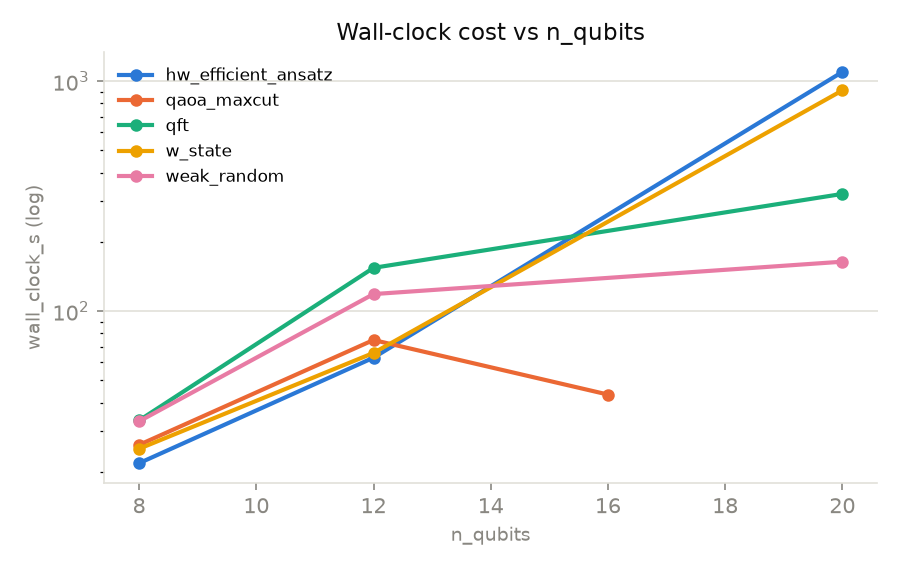
\includegraphics[width=0.75\linewidth]{figures/scaling_wallclock.png}
  \caption{Total wall-clock cost vs.\ qubit count, per circuit family,
    pooled across the three per-block optimizers of the 225-run core
    baseline (log-scaled $y$-axis). Four families grow sharply with
    $n$; \texttt{qaoa\_maxcut}'s three-point trend is not monotonic
    (see discussion above).}
  \label{fig:scaling-wallclock}
\end{figure}

Finally, two structural extensions target
stages this survey's taxonomy does not otherwise cover: reinforcement
learning combined with ZX-calculus~\citep{riu2023rlzx} as an
alternative to the pipeline's hand-rolled compression passes, and
hyperedge-aware partitioning~\citep{sweeney2025hypergraph} in place of
the fixed-modularity Louvain partitioning
Section~\ref{sec:case-study:pipeline} describes. None of these is
implemented in the pipeline today; each is a scoped, independently
addable extension rather than a redesign.

\subsection{Where the Field Appears to Be Heading}
\label{sec:open-challenges:trajectory}

Beyond specific gaps, two recent surveys outside the QIEA-MOO
literature proper suggest where multi-objective optimization as a
whole is heading, for context rather than as a near-term target for
either QIEA-MOO or this survey's case study.
\citet{li2015manyobjective}'s many-objective survey's seven-class
taxonomy (relaxed-dominance, diversity-based, aggregation-based,
indicator-based, reference-set-based, preference-based, and
dimensionality-reduction methods) is a reminder that this survey's own
five classical baselines (Section~\ref{sec:background:moea}) sample
only some of that landscape, and a QIEA-MOO method built around
preference articulation or dimensionality reduction, rather than any of
the five selection paradigms named in
Section~\ref{sec:taxonomy:selection}, remains unexplored.
\citet{doerr2026paretoneural}'s more recent five-level taxonomy --
classical MOEA, ML-guided, RL-driven, LLM-driven, and hybrid
neuro-evolutionary methods -- places every method surveyed in this
paper, and this survey's own case study, at its first level; the field
this taxonomy describes is moving toward learned and neural surrogate
models and RL- or LLM-guided search rather than purely evolutionary
operators, a considerably larger architectural departure than any
single direction in Sections~\ref{sec:open-challenges:methodological}
or~\ref{sec:open-challenges:pipeline} above. We do not read this as a
reason to treat QIEA-MOO or block-partitioned quantum circuit
optimization as obsolete -- both remain useful, interpretable,
comparatively cheap-to-run methods exactly where a learned surrogate's
training cost or data requirement is not justified -- but a
QIEA-MOO method that hybridizes a Q-bit representation with a learned
selection or variation mechanism, rather than only with the classical
selection paradigms surveyed in
Section~\ref{sec:taxonomy:hybridization}, is a direction no method
gathered for this survey has yet taken. Finally,
\citet{zheng2025weakparetoboundary}'s structural critique of
Pareto-dominance-based EMO (Section~\ref{sec:critical-analysis:cross-cutting})
is itself forward-looking as much as critical: a next generation of
QIEA-MOO methods, and of this survey's own case-study pipeline, that
addressed the weak Pareto boundary directly -- rather than continuing to
build on the dominance relation as-is -- would be responding to a
weakness identified in the same year as this survey, not one already
absorbed into current practice.

\section{Conclusion}
\label{sec:conclusion}

Section~\ref{sec:introduction} opened with a gap: quantum-inspired
evolutionary algorithms have been applied to multi-objective problems
since at least \citet{kim2006qmea}'s quantum-inspired multi-objective
knapsack algorithm, yet no prior survey had taxonomized or critically
compared QIEA-for-MOO methods on their own terms, separately from
single-objective QIEA work on one side and classical MOO on the other.
This survey addressed that gap directly. Section~\ref{sec:taxonomy}
organized the literature identified in
Section~\ref{sec:introduction:scope} along five axes -- representation
scheme, quantum-inspired operator type, selection and diversity
mechanism, hybridization with classical MOEAs, and application domain.
Section~\ref{sec:feature-comparison} applied those axes systematically
across the surveyed methods, and in doing so surfaced a pattern the
taxonomy alone had only implied: an overwhelming concentration on
NSGA-II's crowding distance as the selection mechanism of choice, and a
benchmarking culture in which every method is compared against that
same classical baseline but never against its own QIEA-MOO siblings.
Section~\ref{sec:critical-analysis} traced that pattern, and several
others like it, into per-category weaknesses and three cross-cutting
problems -- reproducibility gaps, weak benchmarking practices, and
scalability claims rarely stress-tested -- that recur across the field
regardless of which taxonomy category a given method falls into.

Section~\ref{sec:case-study} grounded several of these abstract claims
in a concrete worked example: this project's own block-partitioned
quantum-circuit-optimization pipeline, itself a direct extension of
\citet{ghlib2026scalable}'s scalable, block-partitioned NSGA-II
framework. We want to restate plainly what that case study was and was
not. It was illustrative -- a way to show, with a real,
actively-maintained codebase, what a swappable selection mechanism
looks like in practice, how an adaptive hypervolume computation can
silently mislead a cross-algorithm comparison, and how easily a
reproducibility gap can hide even inside careful, tested development.
It was not this survey's primary evidence, and none of its numbers
should be read as a benchmark result for QIEA-MOO methods themselves,
which the case study's own pipeline does not use. Full empirical
validation of that pipeline -- including the mutation-scheme and
hybrid-local-search ablations Section~\ref{sec:case-study:mutation}
explicitly left unresolved, pending re-verification on the pipeline's
corrected code -- is the responsibility of a separate, forthcoming
empirical results paper, not this one.

Section~\ref{sec:open-challenges} closed by turning the critical
analysis forward rather than only backward: untested pairings between
the Q-bit representation and selection mechanisms beyond NSGA-II's,
a still-undemonstrated interference-based operator, concrete extensions
to the case-study pipeline drawn from adjacent quantum-computing
literature, and the wider field's movement toward learned and
neural-guided search that neither QIEA-MOO nor this survey's case study
has yet engaged with. None of these close the gap this survey opened
with; each narrows it. If the motivation from
Section~\ref{sec:introduction} is taken seriously -- that a cheaper,
shallower optimization process is not merely a performance metric but
part of a broader case for energy-efficient
computing~\citep{banciu2026aiot,moga2025rlmicrogrid} -- then QIEA-MOO's
comparative youth as a subfield, documented throughout this survey, is
better read as room to grow into than as a reason for caution.


\bibliographystyle{unsrtnat}
\bibliography{references}

\end{document}
